\documentclass{article}
\usepackage[utf8]{inputenc}
\usepackage[spanish]{babel}
\usepackage{graphicx}
\usepackage{amsmath}
\title{Modelos matemáticos discretos}
\author{Susana lizbeth Rodríguez Espinosa}
\begin{document}
\maketitle
\section{Ecuaciones en Diferencias}
\subsection{Primer orden}
Sabemos que $$\lim_{x\to\infty}\frac{1}{x}=0$$

Calcular los valores propios de $$A=
\begin{pmatrix}
1 & 2\\
\pi & 4
\end{pmatrix}.
$$

Consideremos el valor de una inversion de \$1000 que acumula interés de 1\% cada mes.

El valor de la inversión cuando han trancurrido $n$ meses es $$x_n=1000(1.01)^n$$

Una gráfica del resultado es:

\begin{center}
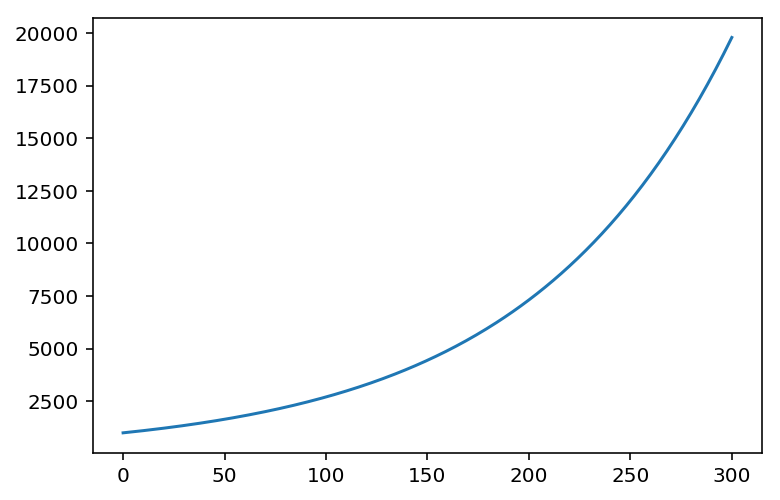
\includegraphics[width=8cm]{grafica}
\end{center}

Para encontrar este resultado, ocupamos que:
$$\sum_{i=0}^{n-1}a^i=\frac{1-a^{n}}{1-a}$$

La ecuación $x_(n+1)=ax_n+b$ se llama una ecuación en diferencias de primer orden lineal con coeficientes constantes no homogénea
Algunos valores de la inversión:
\begin{center}
\begin{tabular}{|c|r|}
\hline
\hline
Mes & Valor\\
\hline
0 & 1000\\
1 & 1010\\
2 & 1021.1\\
3 & 1030.301\\
\hline
\end{tabular}
\end{center}


\begin{center}
\huge
\textbf{NIños no hagan esto en casa}
\end{center}

\subsection{Segundo orden}
\end{document}
